% ****** Start of file apssamp.tex ******
%
%   This file is part of the APS files in the REVTeX 4.2 distribution.
%   Version 4.2a of REVTeX, December 2014
%
%   Copyright (c) 2014 The American Physical Society.
%
%   See the REVTeX 4 README file for restrictions and more information.
%
% TeX'ing this file requires that you have AMS-LaTeX 2.0 installed
% as well as the rest of the prerequisites for REVTeX 4.2
%
% See the REVTeX 4 README file
% It also requires running BibTeX. The commands are as follows:
%
%  1)  latex apssamp.tex
%  2)  bibtex apssamp
%  3)  latex apssamp.tex
%  4)  latex apssamp.tex
%
\documentclass[%
 reprint,
%superscriptaddress,
%groupedaddress,
%unsortedaddress,
%runinaddress,
%frontmatterverbose, 
%preprint,
%preprintnumbers,
%nofootinbib,
%nobibnotes,
%bibnotes,
 amsmath,amssymb,
 aps,
 prd,
%prb,
%rmp,
%prstab,
%prstper,
%floatfix,
]{revtex4-2}

\usepackage{graphicx}% Include figure files
\usepackage{dcolumn}% Align table columns on decimal point
%\usepackage{bm}% bold math
%\usepackage{hyperref}% add hypertext capabilities
%\usepackage[mathlines]{lineno}% Enable numbering of text and display math
%\linenumbers\relax % Commence numbering lines

%\usepackage[showframe,%Uncomment any one of the following lines to test 
%%scale=0.7, marginratio={1:1, 2:3}, ignoreall,% default settings
%%text={7in,10in},centering,
%%margin=1.5in,
%%total={6.5in,8.75in}, top=1.2in, left=0.9in, includefoot,
%%height=10in,a5paper,hmargin={3cm,0.8in},
%]{geometry}

\usepackage{newtxtext}
%\usepackage{newtxmath}
\usepackage[subscriptcorrection,nofontinfo]{mtpro2}
\usepackage[scr=rsfs]{mathalfa}
\usepackage{physics}
\usepackage[shortlabels]{enumitem}
\usepackage{url}
\usepackage{cleveref}


\begin{document}

\preprint{APS/123-QED}

\title{Evolving a Single Puncture Using the Moving Puncture Method}% Force line breaks with \\
\thanks{A footnote to the article title}%

\author{Ann Author}
 \altaffiliation[Also at ]{Physics Department, XYZ University.}%Lines break automatically or can be forced with \\
\author{Second Author}%
 \email{Second.Author@institution.edu}
\affiliation{%
 Authors' institution and/or address\\
 This line break forced with \textbackslash\textbackslash
}%

\collaboration{MUSO Collaboration}%\noaffiliation

\author{Charlie Author}
 \homepage{http://www.Second.institution.edu/~Charlie.Author}
\affiliation{
 Second institution and/or address\\
 This line break forced% with \\
}%
\affiliation{
 Third institution, the second for Charlie Author
}%
\author{Delta Author}
\affiliation{%
 Authors' institution and/or address\\
 This line break forced with \textbackslash\textbackslash
}%

\collaboration{CLEO Collaboration}%\noaffiliation

\date{\today}% It is always \today, today,
             %  but any date may be explicitly specified

\begin{abstract}
In this paper, we investigate the evolution of a single puncture within the framework of the Moving Puncture Method. The Moving Puncture Method has proven to be a powerful technique in numerical relativity for evolving black hole spacetimes. In our study, we focus on its application to the evolution of a single puncture, which can serve as a fundamental building block in simulating more complex spacetime scenarios.
\begin{description}
\item[Usage]
Secondary publications and information retrieval purposes.
\item[Structure]
You may use the \texttt{description} environment to structure your abstract;
use the optional argument of the \verb+\item+ command to give the category of each item. 
\end{description}
\end{abstract}

%\keywords{Suggested keywords}%Use showkeys class option if keyword
                              %display desired
\maketitle

%\tableofcontents

%\section{Introduction}
%Since the first succeeded simulations of merging black-hole binaries to compute accurate gravitational waveforms form, the formulations or techniques used in the simulation such as BSSN(\textit{Baumgarte-Shapiro-Shibata-Nakmura}) formulation \cite{Nakamura:1987,  Shibata:1995we, Baumgarte:1998te}, conformal decompositions \cite{PhysRevLett.26.1656, Lichnerowicz:1944zz}, Bowen-York approach \cite{Bowen:1980yu} and moving puncture gauge \cite{PhysRevD.77.024027} have been used until recently.
%
%Evolving a schwarzschild black hole is good to see how numerical codes works, since we know its analytic solutions.
%
%In this paper, we present the way to get analytic solutions to schwarzschild black hole in case of time-independent. We present numerical setups and results as comparison to analytic solutions.

\section{Introduction}
Since the first successful simulations of merging black-hole binaries for computing accurate gravitational waveforms, various formulations and techniques have been employed. These include the BSSN (\textit{Baumgarte-Shapiro-Shibata-Nakamura}) formulation \cite{Nakamura:1987, Shibata:1995we, Baumgarte:1998te}, conformal decompositions \cite{PhysRevLett.26.1656, Lichnerowicz:1944zz}, the Bowen-York approach \cite{Bowen:1980yu}, and the moving puncture gauge \cite{PhysRevD.77.024027}. These methods have been in use until recently.

Evolving a Schwarzschild black hole serves as a valuable benchmark for assessing the performance of numerical codes, given that we possess its analytical solutions.

In this paper, we present a method for obtaining analytic solutions for a Schwarzschild black hole under time-independent conditions. We provide numerical setups and results for comparison with these analytical solutions.


%\section{Initial data}
%\subsection{Spatial metric}
%We need to specify the spatial metric $\gamma_{ij}$ and the extrinsic curvature $K_{ij}$ which satisfy the Hamiltonian constraint
%\begin{equation}
%	\label{eq:ham}
%	R + K^2 - K_{ij}K^{ij} = 16 \pi \rho,
%\end{equation}
%and the momentum constraint
%\begin{equation}
%	\label{eq:mom}
%	D_j(K^{ij} - \gamma^{ij}K) = 8\pi j^i.
%\end{equation}
%
%To construct a single puncture initial data, we adopt York-Lichnerowicz conformal decompositions \cite{PhysRevLett.26.1656, Lichnerowicz:1944zz}. The spatial metric is decomposed into a conformal factor $\psi$ multiplying an conformally related metric:
%\begin{equation}
%	\label{eq:conformalmetric}
%	\gamma_{ij} = \psi^4 \bar{\gamma}_{ij}.
%\end{equation}
%With this, \eqref{eq:ham} turns into
%\begin{equation}
%	\label{eq:conham}
%	\bar{D}^2\psi - \frac{\psi}{8}\bar{R}+\frac{\psi^5}{8}\qty(K_{ij}K^{ij}-K^2)=-2\pi \psi^5 \rho,
%\end{equation}
%where we define the conformal Laplace operator
%\begin{equation}
%	\bar{D}^2\psi \equiv \bar{\gamma}^{ij}\bar{D}_i\bar{D}_j \psi.
%\end{equation}
%We assume
%\begin{enumerate}[1)]
%	\item \textit{vacuum spacetime} ($\rho = 0$, $j^i = 0$),
%	\item \textit{time symmetry} ($\partial_t \gamma_{ij} = 0$, $\beta^i = 0$),
%\end{enumerate}
%so the extrinsic curvature
%\begin{equation}
%	K_{ij} = \frac{1}{2\alpha}\qty(\mathcal{L}_\beta \gamma_{ij} - \partial_t \gamma_{ij})
%\end{equation}
%vanishes and also $K=0$. Therefore, \eqref{eq:mom} satisfied identically. If we assume \textit{conformal flatness}, the conformally related metric to be flat,
%\begin{equation}
%	\bar{\gamma}_{ij} = \eta_{ij},
%\end{equation}
%\eqref{eq:conham} reduces to the simple Laplace equation
%\begin{equation}
%	\bar{D}^2\psi = 0,
%\end{equation}
%which has the solution
%\begin{equation}
%	\psi = A + \frac{B}{r}.
%\end{equation}
%To satisfy asymptotically flat as $r\to \infty$, and ADM mass to be $M$, we should choose $A=1$ and $B=\frac{M}{2}$:
%\begin{equation}
%	\label{eq:psi}
%	\psi = 1 + \frac{M}{2r}.
%\end{equation}

\section{Initial data}
\subsection{Spatial Metric}
We need to specify the spatial metric $\gamma_{ij}$ and the extrinsic curvature $K_{ij}$ which satisfy the Hamiltonian constraint
\begin{equation}
	\label{eq:ham}
	R + K^2 - K_{ij}K^{ij} = 16 \pi \rho,
\end{equation}
and the momentum constraint
\begin{equation}
	\label{eq:mom}
	D_j(K^{ij} - \gamma^{ij}K) = 8\pi j^i.
\end{equation}

To construct a single puncture initial data, we adopt York-Lichnerowicz conformal decompositions \cite{PhysRevLett.26.1656, Lichnerowicz:1944zz}. The spatial metric is decomposed into a conformal factor $\psi$ multiplying an conformally related metric:
\begin{equation}
	\label{eq:conformalmetric}
	\gamma_{ij} = \psi^4 \bar{\gamma}_{ij}.
\end{equation}
With this, \eqref{eq:ham} turns into
\begin{equation}
	\label{eq:conham}
	\bar{D}^2\psi - \frac{\psi}{8}\bar{R}+\frac{\psi^5}{8}\qty(K_{ij}K^{ij}-K^2)=-2\pi \psi^5 \rho,
\end{equation}
where we define the conformal Laplace operator
\begin{equation}
	\bar{D}^2\psi \equiv \bar{\gamma}^{ij}\bar{D}_i\bar{D}_j \psi.
\end{equation}
We assume
\begin{enumerate}[1)]
	\item \textit{vacuum spacetime} ($\rho = 0$, $j^i = 0$),
	\item \textit{time symmetry} ($\partial_t \gamma_{ij} = 0$, $\beta^i = 0$),
\end{enumerate}
so the extrinsic curvature
\begin{equation}
	K_{ij} = \frac{1}{2\alpha}\qty(\mathcal{L}_\beta \gamma_{ij} - \partial_t \gamma_{ij})
\end{equation}
vanishes and also $K=0$. Therefore, \eqref{eq:mom} satisfied identically. If we assume \textit{conformal flatness}, the conformally related metric to be flat,
\begin{equation}
	\bar{\gamma}_{ij} = \eta_{ij},
\end{equation}
\eqref{eq:conham} reduces to the simple Laplace equation
\begin{equation}
	\bar{D}^2\psi = 0,
\end{equation}
which has the solution
\begin{equation}
	\psi = A + \frac{B}{r}.
\end{equation}
To satisfy asymptotically flat as $r\to \infty$, and ADM mass to be $M$, we should choose $A=1$ and $B=\frac{M}{2}$:
\begin{equation}
	\label{eq:psi}
	\psi = 1 + \frac{M}{2r}.
\end{equation}

%
%\textsc{TwoPunctures} \cite{Ansorg:2004ds} use Bowen-York approach \cite{Bowen:1980yu} and using method in \cite{PhysRevD.77.024027}. Since there is a single puncture with neither spin nor momentum, the result should be same as \eqref{eq:psi}. We used \texttt{TP_epsilon} to $10^{-6}$ and \texttt{TP_Tiny} to $0$, so
%\begin{equation}
%	\psi = 1 + \frac{M}{2\tilde{r}},
%\end{equation}
%where
%\begin{equation}
%	\tilde{r} = \qty(r^4 + 10^{-24})^{1/4}.
%\end{equation}
%
%The initial metric set by \textsc{TwoPunctures} exactly has the form
%\begin{equation}
%	\gamma_{ij} = \qty(1 + \frac{M}{2\tilde{r}})^4\eta_{ij},
%\end{equation}
%for all grid points. Fig.~\ref{fig:gammaxx} shows $\gamma_{xx}$ along $x$ axis at initial time. Each marker represents grid point for refinement level respectively. Non-diagonal component of spatial metric and all component of extrinsic curvature has value of 0 explicitly.
%
%\begin{figure}[h]
%	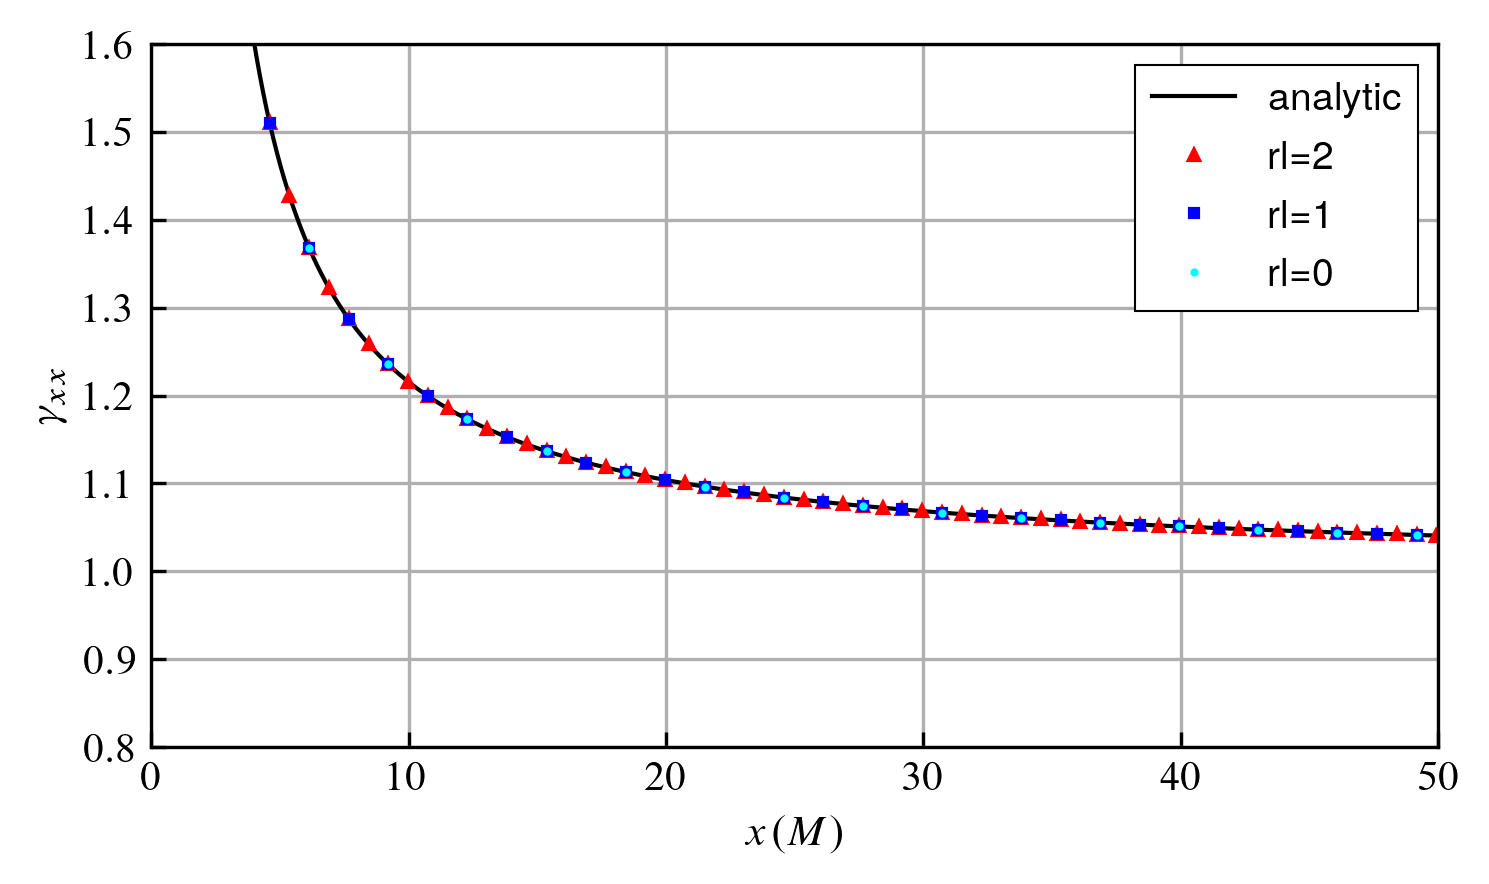
\includegraphics[width=0.5\textwidth]{data/gammaxx.png}% Here is how to import EPS art
%	\caption{\label{fig:gammaxx} $\gamma_{xx}$ along $x$ axis at initial time. Only 3 of 7 refinement level plotted.}
%\end{figure}

\textsc{TwoPunctures} \cite{Ansorg:2004ds} uses the Bowen-York approach \cite{Bowen:1980yu} and the method presented in \cite{PhysRevD.77.024027}. Since there is a single puncture with neither spin nor momentum, the result should be the same as in \eqref{eq:psi}. We set \texttt{TP_epsilon} to $10^{-6}$ and \texttt{TP_Tiny} to $0$, resulting in
\begin{equation}
	\psi = 1 + \frac{M}{2\tilde{r}},
\end{equation}
where
\begin{equation}
	\tilde{r} = \left(r^4 + 10^{-24}\right)^{1/4}.
\end{equation}

The initial metric set by \textsc{TwoPunctures} exactly takes the form
\begin{equation}
	\gamma_{ij} = \left(1 + \frac{M}{2\tilde{r}}\right)^4\eta_{ij},
\end{equation}
for all grid points. Fig.~\ref{fig:gammaxx} shows $\gamma_{xx}$ along the $x$-axis at the initial time. Each marker represents a grid point for a respective refinement level. The non-diagonal components of the spatial metric and all components of the extrinsic curvature have explicit values of 0.

\begin{figure}[h]
	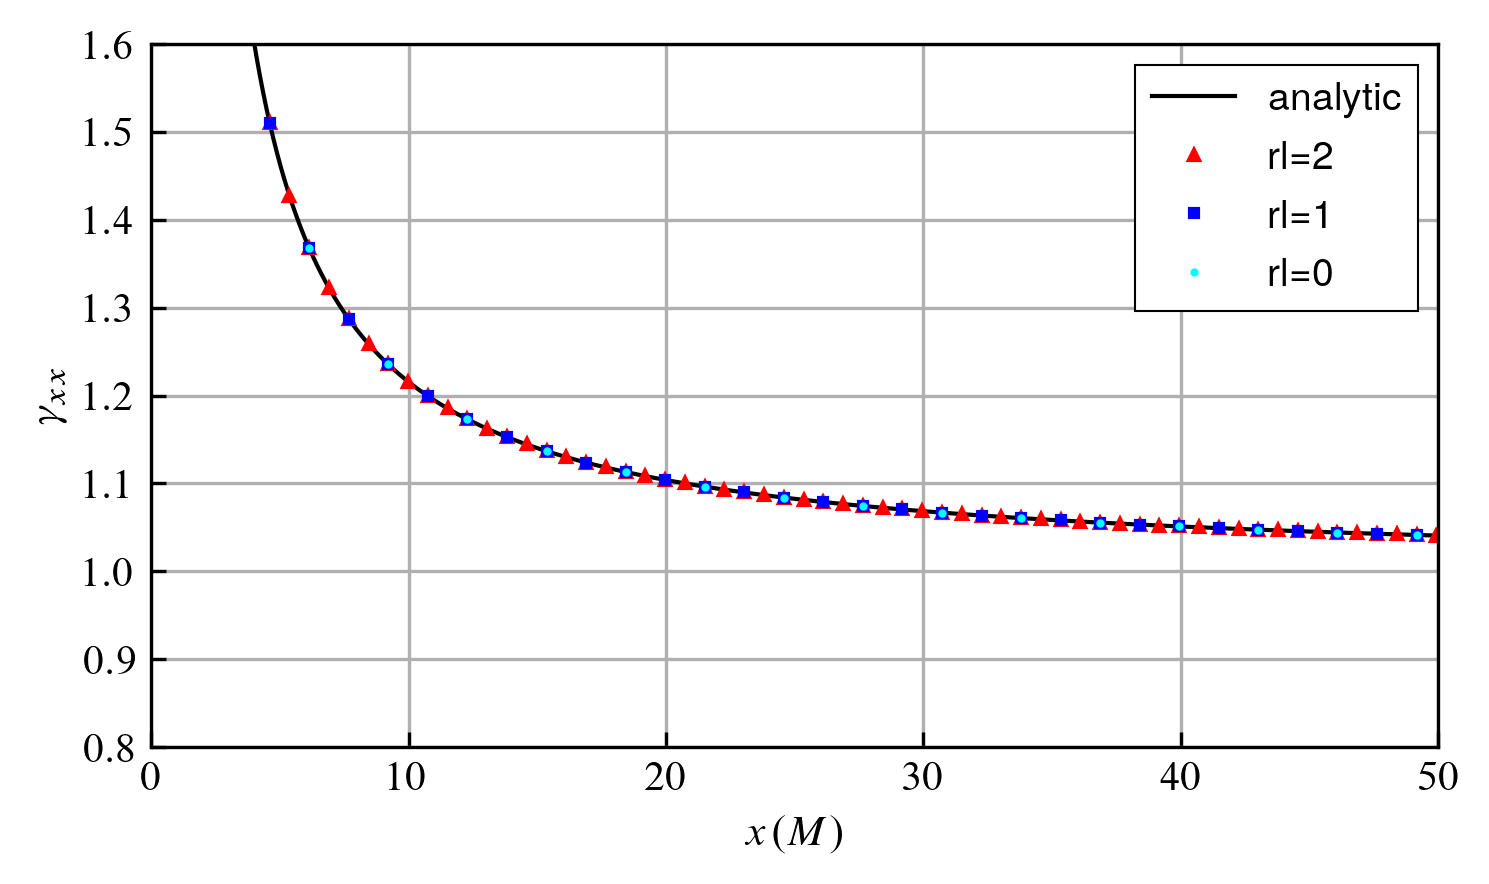
\includegraphics[width=0.5\textwidth]{data/gammaxx.png}% Here is how to import an image
	\caption{\label{fig:gammaxx} $\gamma_{xx}$ along the $x$-axis at the initial time. Only 3 of the 7 refinement levels are plotted.}
\end{figure}

%
%\subsection{Constraints}
%
%From \eqref{eq:ham} and \eqref{eq:mom}, we can define
%\begin{equation}
%	\mathcal{H} \equiv R + K^2 -K_{ij}K^{ij}-16\pi \rho,
%\end{equation}
%\begin{equation}
%	\mathcal{M}^ i \equiv D_j (K^{ij} - \gamma^{ij}K) - 8\pi j^i,
%\end{equation}
%and it should be satisfy that $\mathcal{H} = 0$ and $\mathcal{M}^i = 0$. Fig.~\ref{fig:ham_xy} shows $\log_{10}\qty|\mathcal{H}|$ on the $xy$ plane at the initial time. Every value at each grid points is less than $10^{-7}$. In case of $\mathcal{M}^i$, all of the values are explicitly 0.
%
%\begin{figure}[h]
%	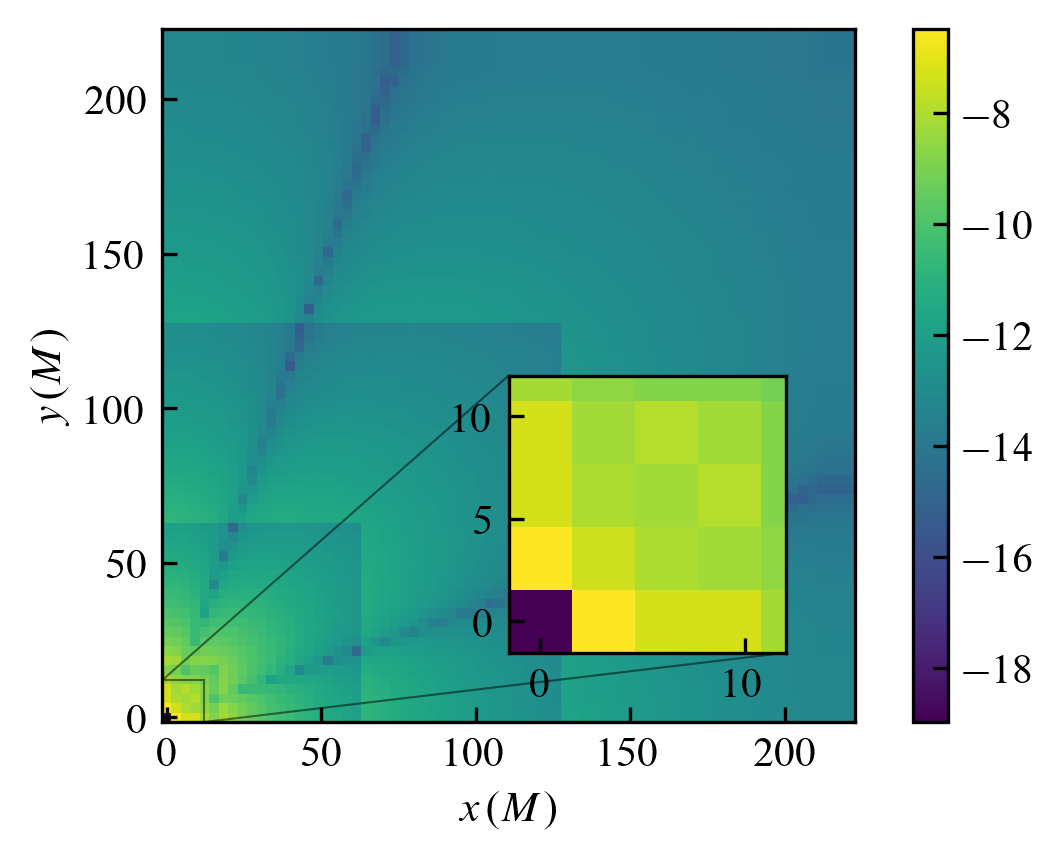
\includegraphics[width=0.5\textwidth]{data/ham_xy.png}% Here is how to import EPS art
%	\caption{\label{fig:ham_xy} $\log_{10}\qty|\mathcal{H}|$ on the $xy$ plane at the initial time.}
%\end{figure}
%
%Fig.~\ref{fig:ham_evol} shows Hamiltonian constraint violation $\mathcal{H}$ along the $x$ axis. The data at $x=0$ has been cut since its value is order of $1$ at the late time. $\mathcal{H}$ increased as time passed and most peak point's $x$ coordinate also increased. But still order of $10^{-6}$ at the $t=115.2M$.
%\begin{figure}[h]
%	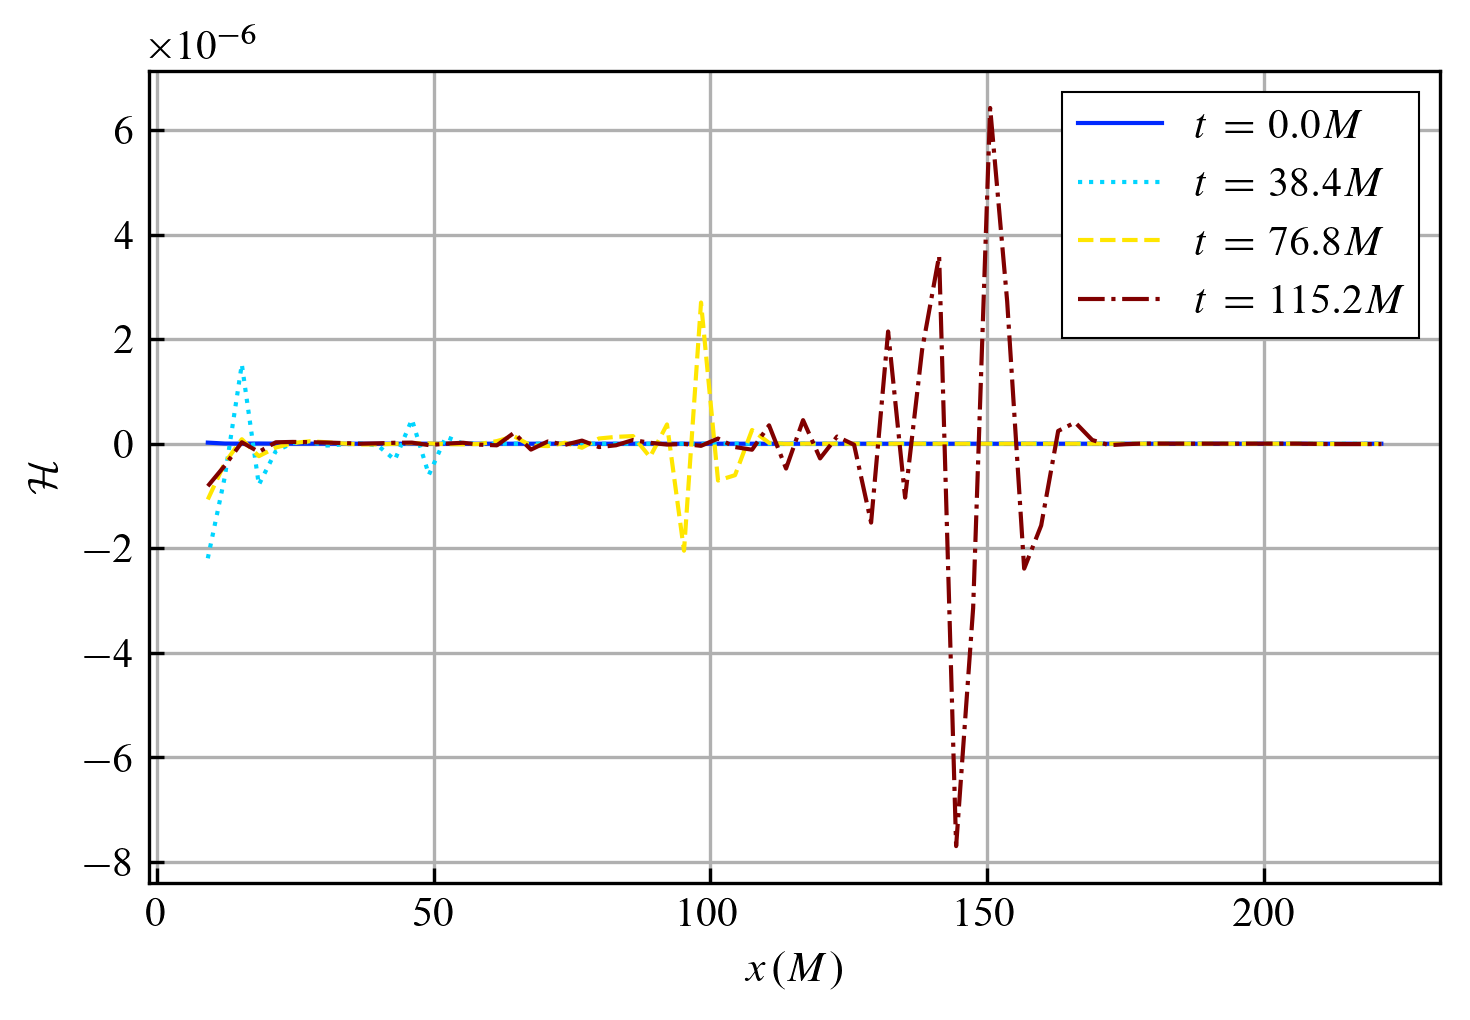
\includegraphics[width=0.5\textwidth]{data/ham_evol.png}% Here is how to import EPS art
%	\caption{\label{fig:ham_evol} The Hamiltonian constraint violation along the $x$ axis.}
%\end{figure}

\subsection{Constraints}

From \eqref{eq:ham} and \eqref{eq:mom}, we can define
\begin{equation}
	\mathcal{H} \equiv R + K^2 - K_{ij}K^{ij} - 16\pi \rho,
\end{equation}
\begin{equation}
	\mathcal{M}^i \equiv D_j (K^{ij} - \gamma^{ij}K) - 8\pi j^i,
\end{equation}
and it should satisfy that $\mathcal{H} = 0$ and $\mathcal{M}^i = 0$. Fig.~\ref{fig:ham_xy} shows $\log_{10}\qty|\mathcal{H}|$ on the $xy$ plane at the initial time. Every value at each grid point is less than $10^{-7}$. In the case of $\mathcal{M}^i$, all of the values are explicitly 0.

\begin{figure}[h]
	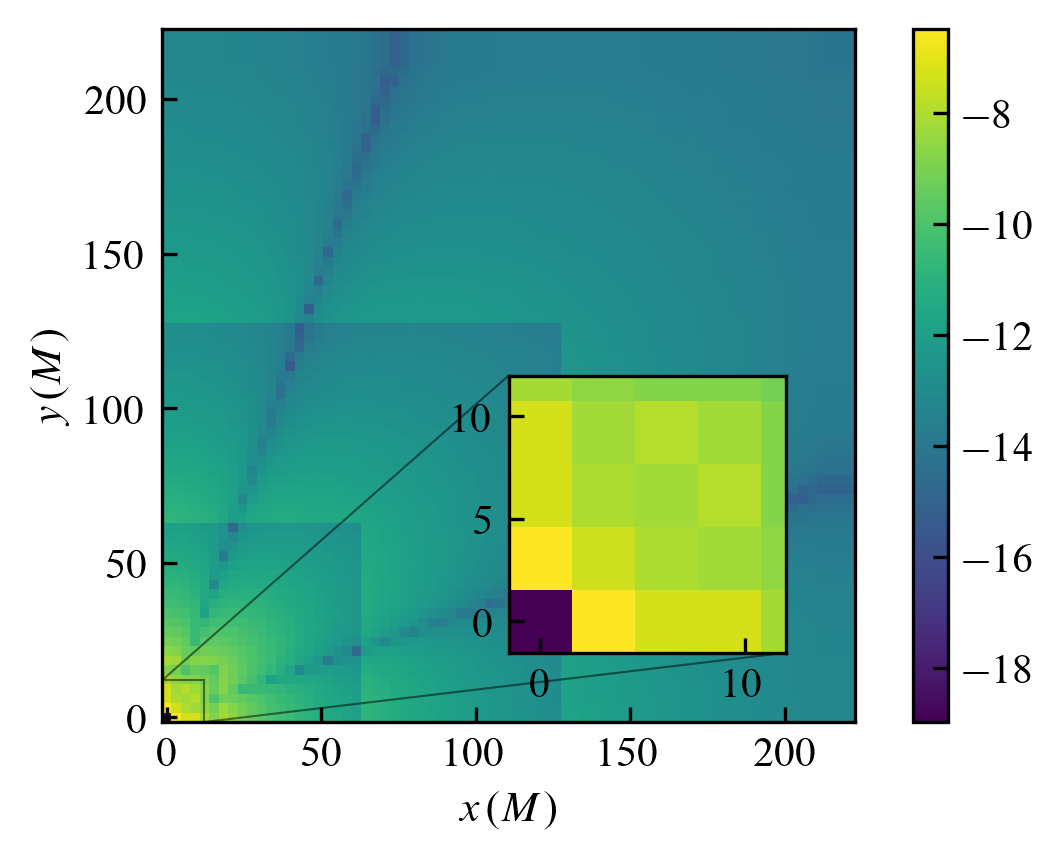
\includegraphics[width=0.5\textwidth]{data/ham_xy.png}% Here is how to import EPS art
	\caption{\label{fig:ham_xy} $\log_{10}\qty|\mathcal{H}|$ on the $xy$ plane at the initial time.}
\end{figure}

Fig.~\ref{fig:ham_evol} shows the Hamiltonian constraint violation $\mathcal{H}$ along the $x$ axis. The data at $x=0$ has been cut since its value is on the order of $1$ at the late time. $\mathcal{H}$ increased as time passed, and most peak point's $x$ coordinate also increased. But it still remains on the order of $10^{-6}$ at $t=115.2M$.
\begin{figure}[h]
	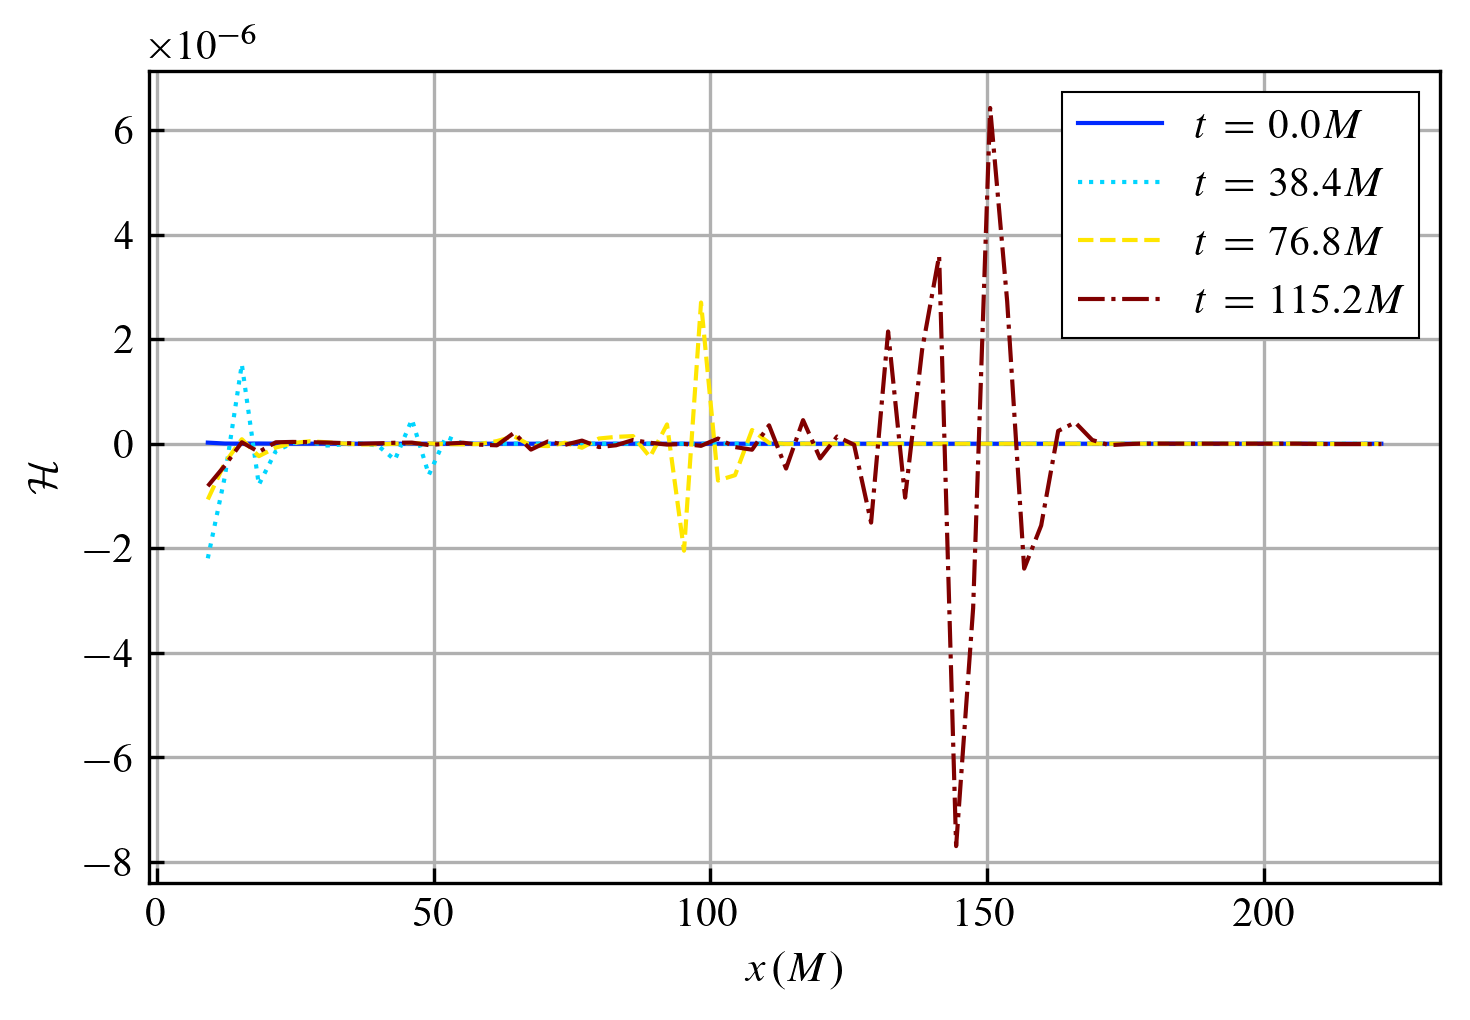
\includegraphics[width=0.5\textwidth]{data/ham_evol.png}% Here is how to import EPS art
	\caption{\label{fig:ham_evol} The Hamiltonian constraint violation along the $x$ axis.}
\end{figure}



%\section{Evolution}
%
%\subsection{Gauge Condition}
%
%The 1+log slicing with advection term is
%\begin{eqnarray}
%	\label{eq:logadv}
%	\partial_t \alpha = -2\alpha K + \beta^i \partial_i \alpha,
%\end{eqnarray}
%and hyperbolic gamma driver condition for the shift with advection term is
%\begin{eqnarray}
%	\label{eq:betaadv}
%	\partial_t \beta^i = \frac{3}{4}B^i + \beta^j\partial_j \beta^i,
%\end{eqnarray}
%\begin{eqnarray}
%	\label{eq:Badv}
%	\partial_t B^i = \partial_t \bar{\Gamma}^i -B^i + \beta^j \partial_j B^i,
%\end{eqnarray}
%which is typically employed in moving puncture method \cite{Campanelli:2005dd, Alcubierre:2002kk}. Sometimes we can drop advection term so that the \eqref{eq:logadv}, \eqref{eq:betaadv}. \eqref{eq:Badv} becomes
%\begin{eqnarray}
%	\label{eq:lognoadv}
%	\partial_t \alpha = -2\alpha K,
%\end{eqnarray}
%\begin{eqnarray}
%	\label{eq:betanoadv}
%	\partial_t \beta^i = \frac{3}{4}B^i,
%\end{eqnarray}
%\begin{eqnarray}
%	\label{eq:Bnoadv}
%	\partial_t B^i = \partial_t \bar{\Gamma}^i -B^i,
%\end{eqnarray}
%which we adopt this paper.
%
%We used \texttt{twopunctures-averaged} initial lapse which given by
%\begin{eqnarray}
%	\alpha &=& \frac{1}{2}(1 + \alpha'),
%\end{eqnarray}
%where
%\begin{eqnarray}
%	\alpha' &=& \frac{1 - \frac{M}{2r}}{1 + \frac{M}{2r}},
%\end{eqnarray}
%therefore lapse satisfy $0 \le \alpha \le 1$.
%
%When the simulation goes sufficiently and the solution becomes time-independent, it must be $\partial_t \alpha = 0$, implying $K=0$. Since we choose hyperbolic gamma driver condition, it has special solution (see \cite{PhysRevD.75.067502, PhysRevD.78.064020})
%\begin{eqnarray}
%	\label{eq:alpha}
%	\alpha = \qty(1 - \frac{2M}{r_s} + \frac{27M^4}{16r_s^4})^{1/2}.
%\end{eqnarray}
%$r_s$ is an areal radius and it is related with isotropic radius $r$ as
%\begin{widetext}
%\begin{eqnarray}
%	\label{eq:rtors}
%	r &=& \frac{2r_s + M + (4r_s^2 +4Mr_s+3M^2)^{1/2}}{4}\times \qty(\frac{(4+3\sqrt{2})(2r_s - 3M)}{8r_s + 6M + 3 (8r_s^2 + 8Mr_s+6M^2)^{1/2}})^{1/\sqrt{2}}.
%\end{eqnarray}
%\end{widetext}
%
%The conformal factor is given by $\psi = \qty(\frac{r_s}{r})^{1/2}$, and substitute \eqref{eq:rtors},
%\begin{widetext}
%\begin{eqnarray}
%	\label{eq:psi_long}
%	\psi = \qty(\frac{4r_s}{2r_s + M + (4r_s^2 + 4Mr_s + 3M^2)^{1/2}})^{1/2}\qty(\frac{8r_s + 6M + 3 (8r_s^2 + 8Mr_s + 6M^2)^{1/2}}{(4+3\sqrt{2})(2r_s - 3M)})^{1/2\sqrt{2}}.
%\end{eqnarray}
%\end{widetext}
%
%Fig.~\ref{fig:alphas} shows $\alpha$ along $x$ axis at several times. After $t=49.152M$, $\alpha$ almost static. Black solid line indicates analytic solution given as \eqref{eq:alpha}.
%\begin{figure}[h]
%	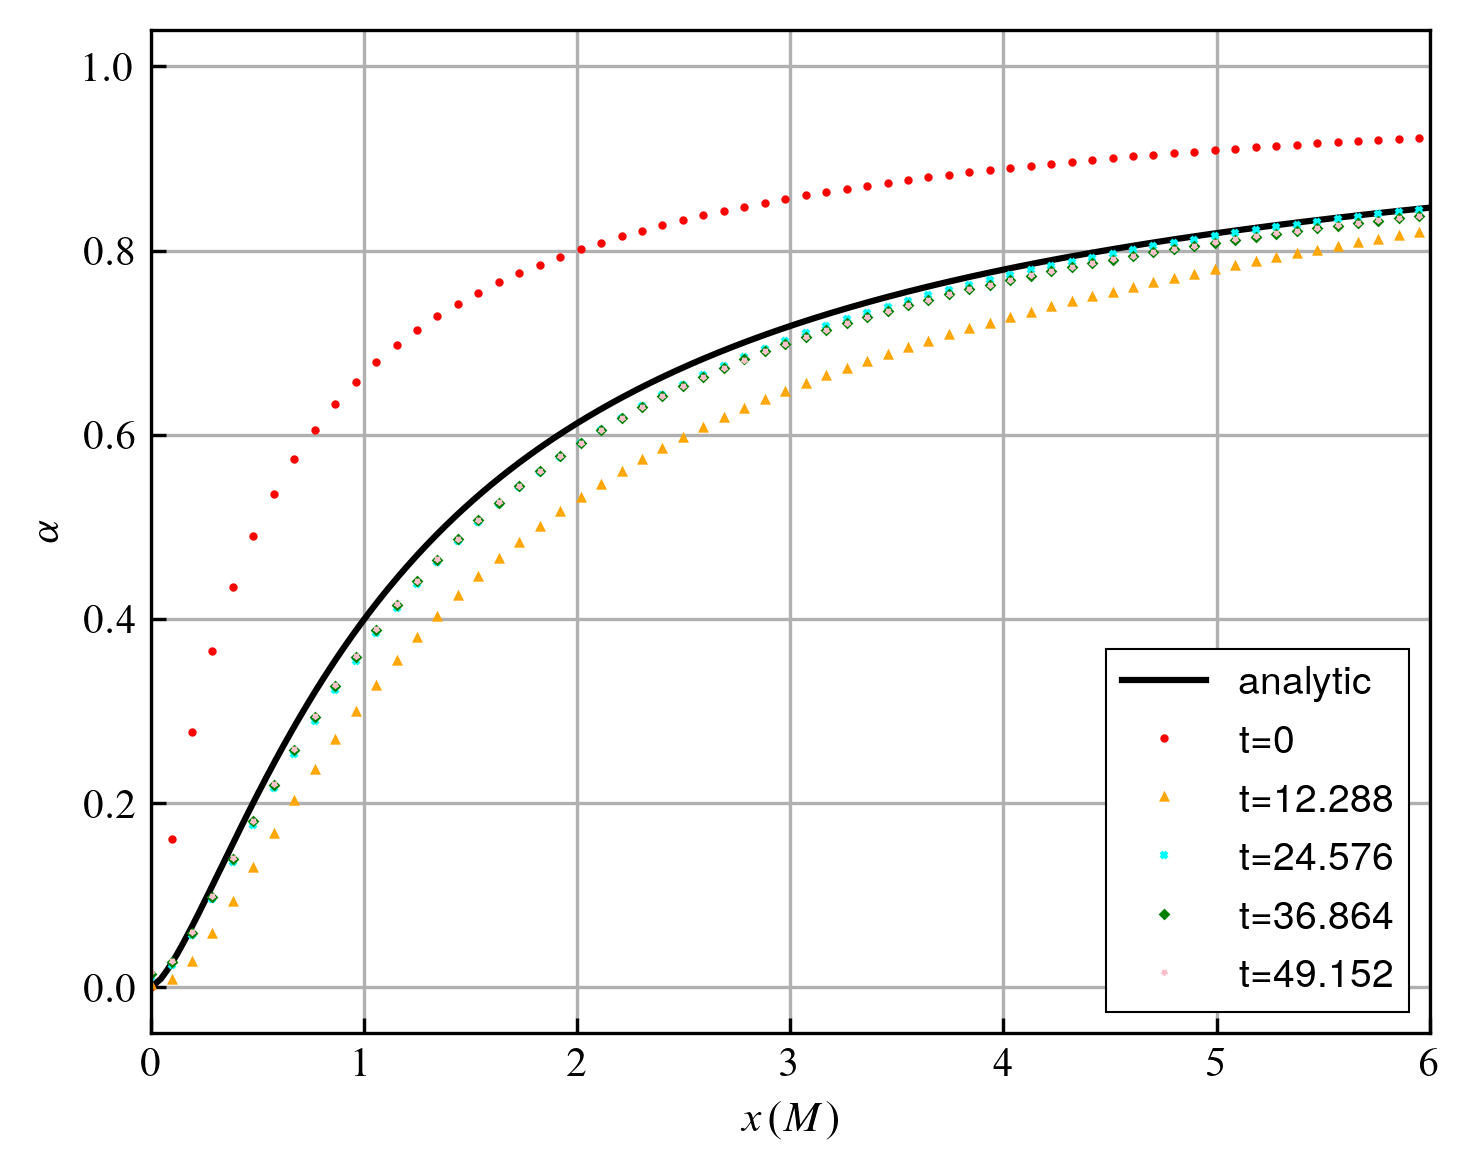
\includegraphics[width=0.5\textwidth]{data/alphas.png}% Here is how to import EPS art
%	\caption{\label{fig:alphas} $\alpha$ along $x$ axis at several times. Only 5 refinement level plotted. Time unit is divided by $M$.}
%\end{figure}
%
%Fig.~\ref{fig:ev_gammaxx} shows $\gamma_{xx}$ along $x$ axis. The black solid line indicates analytic solution $\gamma_{ij} = \psi^4 \eta_{ij}$, where $\psi$ is given by \eqref{eq:psi_long}.
%
%\begin{figure}[h]
%	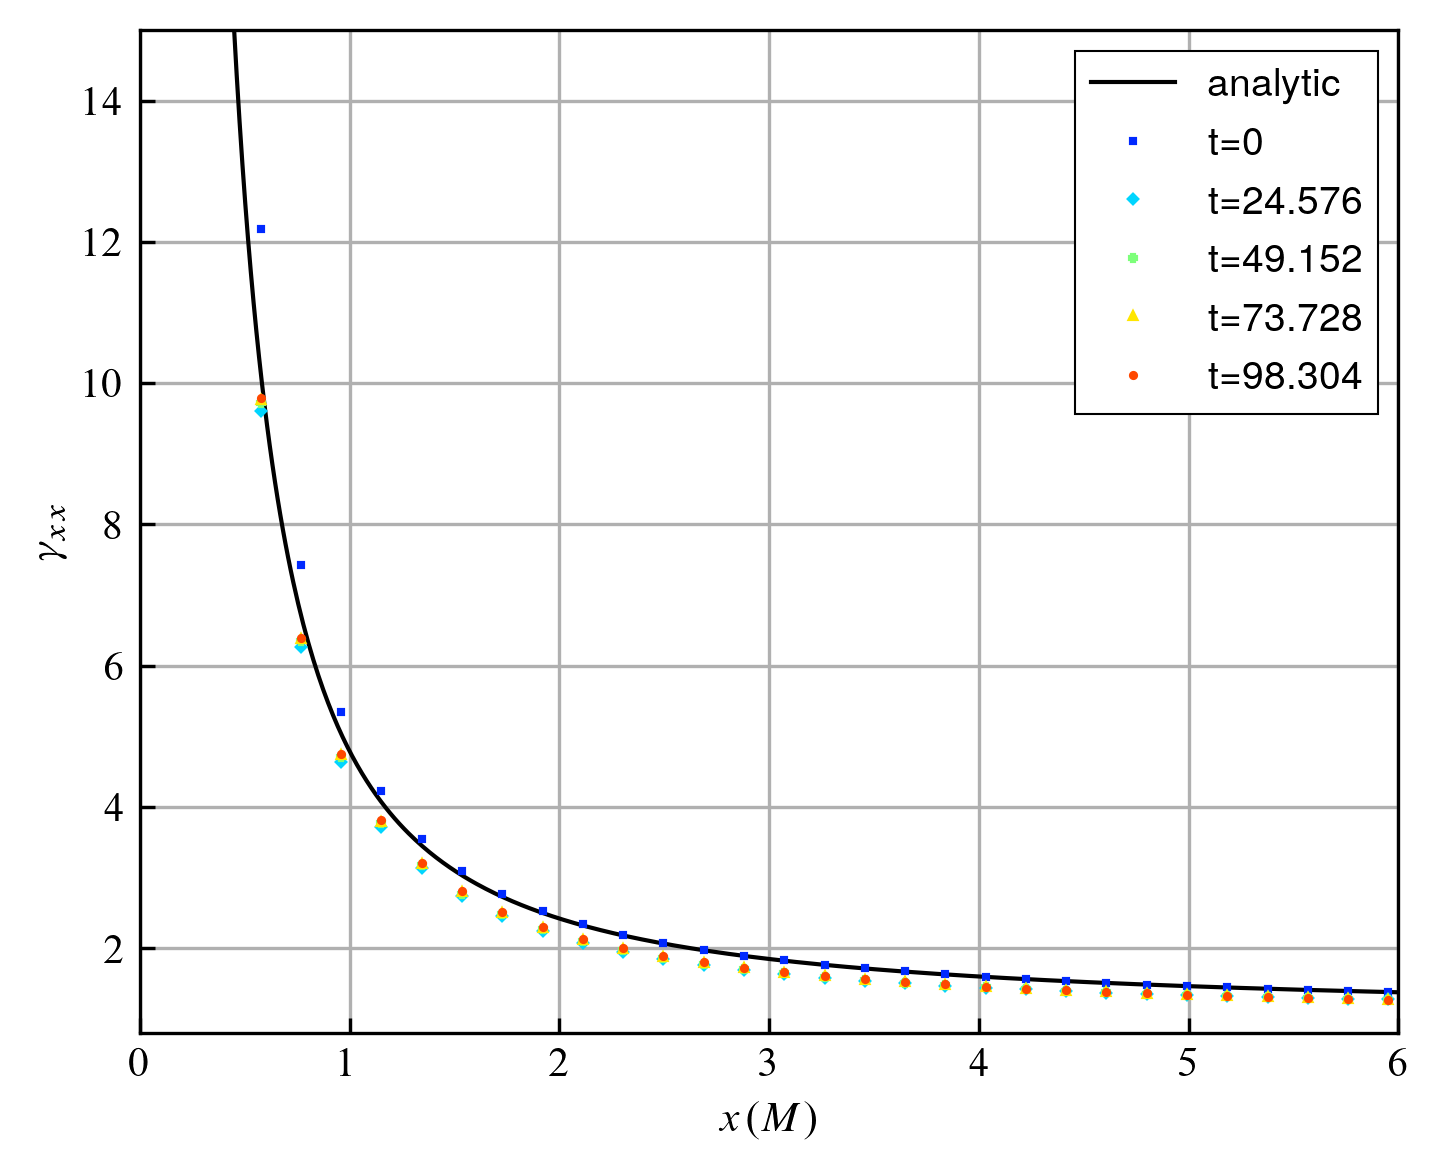
\includegraphics[width=0.5\textwidth]{data/ev_gammaxx.png}% Here is how to import EPS art
%	\caption{\label{fig:ev_gammaxx} $\gamma_{xx}$ along $x$ axis at several times. Only refinement level 4 plotted. Time unit is divided by $M$.}
%\end{figure}

\section{Evolution}

\subsection{Gauge Condition}

The 1+log slicing with advection term is given by
\begin{eqnarray}
	\label{eq:logadv}
	\partial_t \alpha = -2\alpha K + \beta^i \partial_i \alpha,
\end{eqnarray}
and the hyperbolic gamma driver condition for the shift with advection term is defined as
\begin{eqnarray}
	\label{eq:betaadv}
	\partial_t \beta^i = \frac{3}{4}B^i + \beta^j\partial_j \beta^i,
\end{eqnarray}
\begin{eqnarray}
	\label{eq:Badv}
	\partial_t B^i = \partial_t \bar{\Gamma}^i -B^i + \beta^j \partial_j B^i,
\end{eqnarray}
which is typically employed in the moving puncture method \cite{Campanelli:2005dd, Alcubierre:2002kk}. Sometimes we can drop the advection term, simplifying \eqref{eq:logadv}, \eqref{eq:betaadv}, and \eqref{eq:Badv} to
\begin{eqnarray}
	\label{eq:lognoadv}
	\partial_t \alpha = -2\alpha K,
\end{eqnarray}
\begin{eqnarray}
	\label{eq:betanoadv}
	\partial_t \beta^i = \frac{3}{4}B^i,
\end{eqnarray}
\begin{eqnarray}
	\label{eq:Bnoadv}
	\partial_t B^i = \partial_t \bar{\Gamma}^i -B^i,
\end{eqnarray}
which we adopt in this paper.

We used the \texttt{twopunctures-averaged} initial lapse, which is given by
\begin{eqnarray}
	\alpha &=& \frac{1}{2}(1 + \alpha'),
\end{eqnarray}
where
\begin{eqnarray}
	\alpha' &=& \frac{1 - \frac{M}{2r}}{1 + \frac{M}{2r}},
\end{eqnarray}
ensuring that the lapse satisfies $0 \le \alpha \le 1$.

When the simulation progresses sufficiently, and the solution becomes time-independent, we have $\partial_t \alpha = 0$, implying $K=0$. Since we choose the hyperbolic gamma driver condition, it has a special solution (see \cite{PhysRevD.75.067502, PhysRevD.78.064020})
\begin{eqnarray}
	\label{eq:alpha}
	\alpha = \sqrt{1 - \frac{2M}{r_s} + \frac{27M^4}{16r_s^4}},
\end{eqnarray}
where $r_s$ is an areal radius related to the isotropic radius $r$ as
\begin{widetext}
	\begin{eqnarray}
		\label{eq:rtors}
		r &=& \frac{2r_s + M + (4r_s^2 +4Mr_s+3M^2)^{1/2}}{4}\times \left(\frac{(4+3\sqrt{2})(2r_s - 3M)}{8r_s + 6M + 3 (8r_s^2 + 8Mr_s+6M^2)^{1/2}}\right)^{1/\sqrt{2}}.
	\end{eqnarray}
\end{widetext}

The conformal factor is given by $\psi = \left(\frac{r_s}{r}\right)^{1/2}$, and when substituted into \eqref{eq:rtors}, we obtain
\begin{widetext}
	\begin{eqnarray}
		\label{eq:psi_long}
		\psi = \left(\frac{4r_s}{2r_s + M + (4r_s^2 + 4Mr_s + 3M^2)^{1/2}}\right)^{1/2}\left(\frac{8r_s + 6M + 3 (8r_s^2 + 8Mr_s + 6M^2)^{1/2}}{(4+3\sqrt{2})(2r_s - 3M)}\right)^{1/2\sqrt{2}}.
	\end{eqnarray}
\end{widetext}

Fig.~\ref{fig:alphas} shows $\alpha$ along the $x$ axis at several times. After $t=49.152M$, $\alpha$ remains almost constant. The black solid line represents the analytic solution given in \eqref{eq:alpha}.
\begin{figure}[h]
	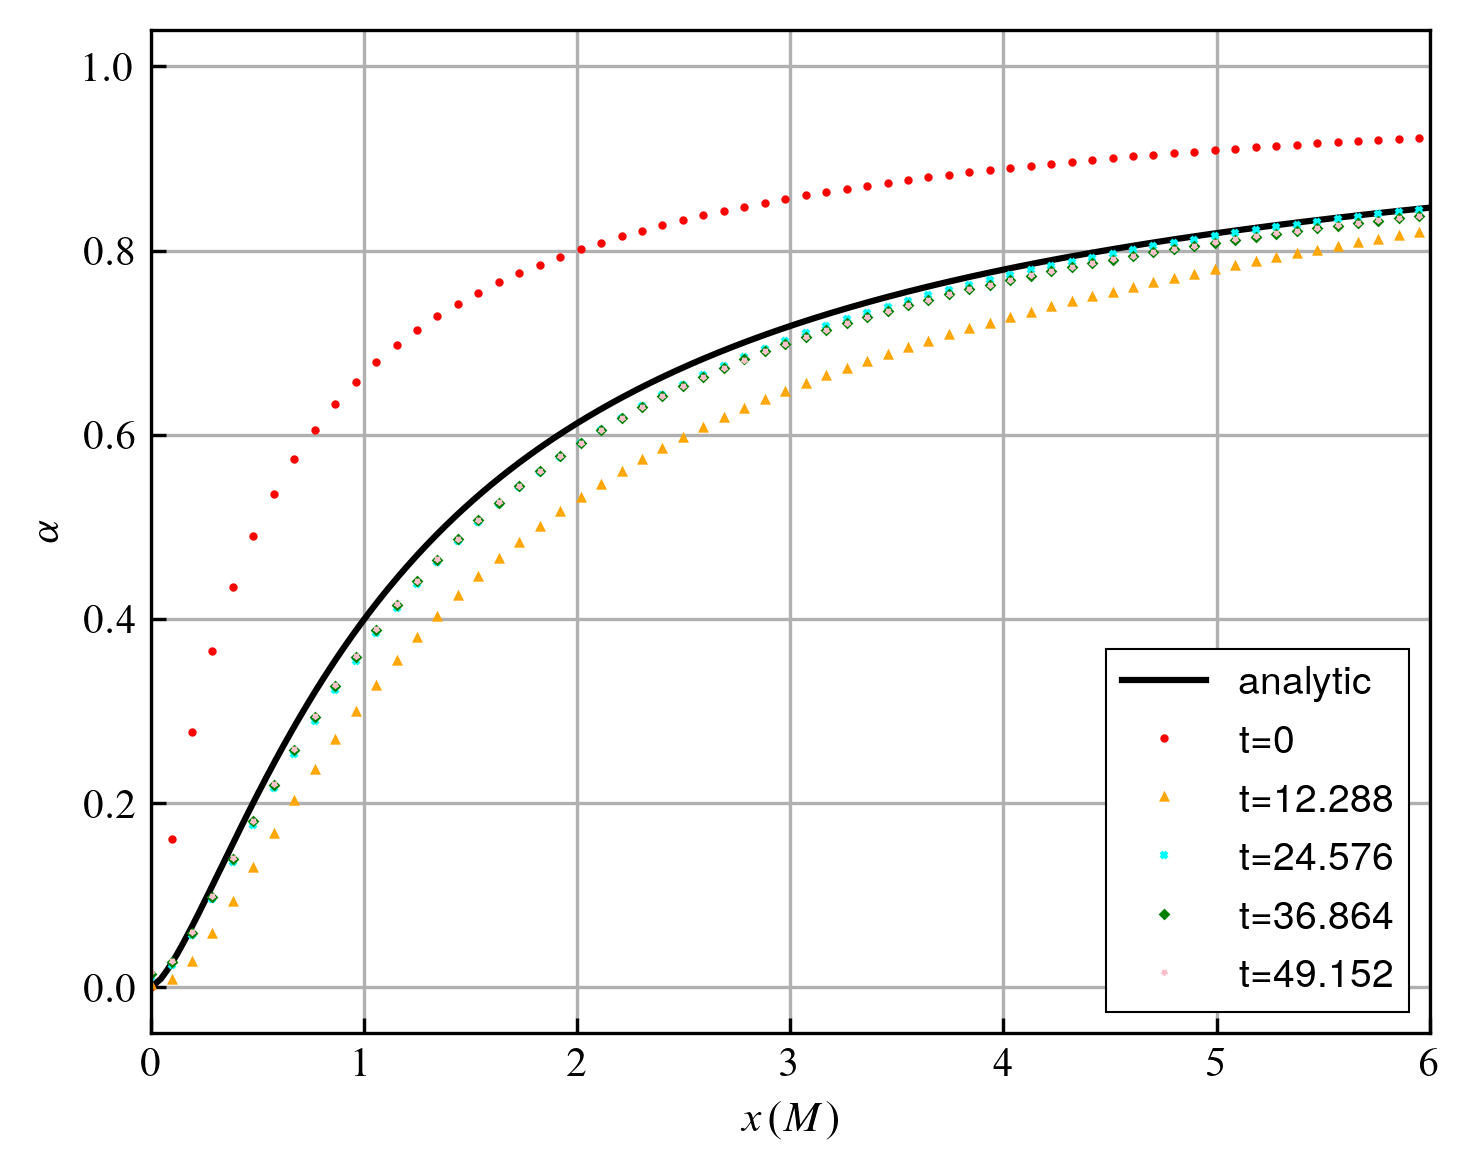
\includegraphics[width=0.5\textwidth]{data/alphas.png}% Here is how to import an image
	\caption{\label{fig:alphas} $\alpha$ along the $x$ axis at several times. Only 5 refinement levels are plotted. The time unit is divided by $M$.}
\end{figure}

Fig.~\ref{fig:ev_gammaxx} shows $\gamma_{xx}$ along the $x$ axis. The black solid line indicates the analytic solution $\gamma_{ij} = \psi^4 \eta_{ij}$, where $\psi$ is given by \eqref{eq:psi_long}.

\begin{figure}[h]
	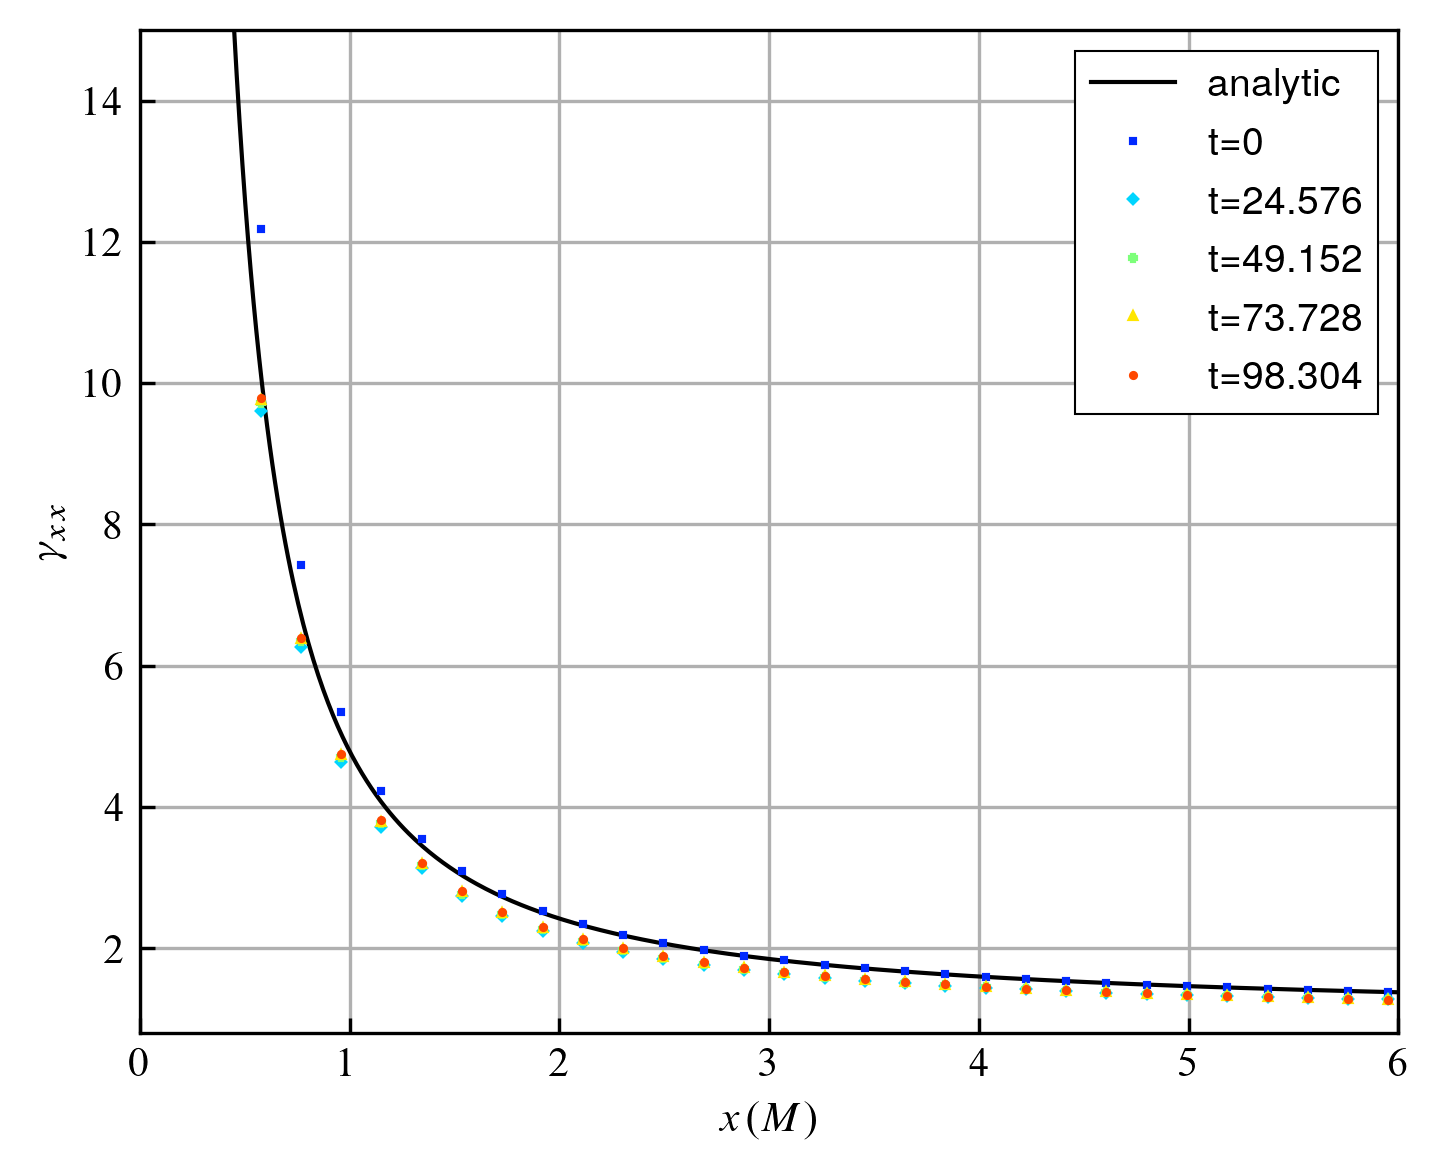
\includegraphics[width=0.5\textwidth]{data/ev_gammaxx.png}% Here is how to import an image
	\caption{\label{fig:ev_gammaxx} $\gamma_{xx}$ along the $x$ axis at several times. Only refinement level 4 is plotted. The time unit is divided by $M$.}
\end{figure}



%\subsection{BSSN}
%The 3+1 ADM evolution equations are
%\begin{equation}
%	(\partial_t - \mathcal{L}_\beta)\gamma_{ij} = -2\alpha K_{ij},
%\end{equation}
%
%\begin{eqnarray}
%	(\partial_t - \mathcal{L}_\beta)K_{ij} &=& -D_i D_j \alpha + \alpha (R_{ij} + KK_{ij}-2K_{ik}K^k{}_{j})\nonumber\\&&+4\pi \alpha M_{ij},
%\end{eqnarray}
%and this set of PDE's is only weakly hyperbolic and is therefore not suitable for stable numerical evolution. Here, we adopt the BSSN(\textit{Baumgarte-Shapiro-Shibata-Nakmura}) formulation \cite{Nakamura:1987,  Shibata:1995we, Baumgarte:1998te}.
%
%In the BSSN formulation, spatial metric $\gamma_{ij}$ is decomposed into conformally related metric as \eqref{eq:conformalmetric} with $\det (\bar{\gamma}_{ij}) = 1$. Extrinsic curvature also decomposed into its trace and traceless parts and conformally transform the traceless part as we do the metric,
%\begin{equation}
%	K_{ij} = e^{4\phi}\tilde{A}_{ij} + \frac{1}{3}\gamma_{ij}K.
%\end{equation}
%We then promote the following variables to evolution variable
%\begin{equation}
%	\phi = \ln \psi = \frac{1}{12}\ln \gamma,
%\end{equation}
%as well as the conformal connection functions
%\begin{equation}
%	\bar{\Gamma}^i = \bar{\gamma}^{jk}\bar{\Gamma}^i{}_{jk} = -\partial_j \bar{\gamma}^{ij}.
%\end{equation}
%Then the evolution equation for $\gamma_{ij}$ splits into two equations,
%\begin{equation}
%	\partial_t \phi = - \frac{1}{6}\alpha K + \beta^i \partial_i \phi + \frac{1}{6}\partial_i \beta^i,
%\end{equation}
%\begin{eqnarray}
%	\label{eq:bssn_gamma}
%	\partial_t \bar{\gamma}_{ij} &=& -2\alpha \tilde{A}_{ij} + \beta^k \partial_k \bar{\gamma}_{ij}  \nonumber\\&&+\bar{\gamma}_{ik}\partial_j \beta^k + \bar{\gamma}_{jk}\partial_i \beta^k - \frac{2}{3}\bar{\gamma}_{ij}\partial_k\beta^k.
%\end{eqnarray}
%And the evolution equation for $K_{ij}$ splits into the two equations,
%\begin{eqnarray}
%	\label{eq:bssn_K}
%\partial_t K &=& -D^iD_i \alpha + \alpha (\tilde{A}_{ij}\title{A}^{ij} + \frac{1}{3}K^2)\nonumber\\&&+\beta^i\partial_i K + 4\pi \alpha (\rho + S),
%\end{eqnarray}
%\begin{eqnarray}
%	\label{eq:bssn_A}
%	\partial_t \tilde{A}_{ij} &=& e^{-4\phi}\qty[-D_iD_j\alpha + \alpha(R_{ij} - 8\pi S_{ij})]^{TF}\nonumber\\&& + \alpha(K\tilde{A}_{ij} - 2\tilde{A}_{ik}\tilde{A}^k{}_{j}) + \beta^k\partial_k \tilde{A}_{ij} \nonumber\\&&+ \tilde{A}_{ik}\partial_j\beta^k + \tilde{A}_{jk}\partial_i\beta^k - \frac{2}{3}\tilde{A}_{ij}\partial_k\beta^k,
%\end{eqnarray}
%where the superscript $TF$ denotes the trace-free part of a tensor. The We also split the Ricci tensor into 
%\begin{eqnarray}
%	R_{ij}
%	&=& \bar{R}_{ij} - 2 \qty(\bar{D}_i\bar{D}_j \ln \psi + \bar{\gamma}_{ij}\bar{\gamma}^{lm}\bar{D}_l \bar{D}_m \ln \psi)\nonumber\\&&+4\qty((\bar{D}_i \ln \psi)(\bar{D}_j \ln \psi) - \bar{\gamma}_{ij}\bar{\gamma}^{lm}(\bar{D}_l \ln \psi)(\bar{D}_m \ln \psi) )\nonumber\\
%	&=& \bar{R}_{ij} - 2 \qty(\bar{D}_i\bar{D}_j \phi + \bar{\gamma}_{ij}\bar{\gamma}^{lm}\bar{D}_l \bar{D}_m \phi)\nonumber\\&&+4\qty((\bar{D}_i \phi)(\bar{D}_j \phi) - \bar{\gamma}_{ij}\bar{\gamma}^{lm}(\bar{D}_l \phi)(\bar{D}_m \phi) )\nonumber\\
%	&\equiv& \bar{R}_{ij} + R^\phi_{ij}.
%\end{eqnarray}
%The $\bar{\Gamma}^{i}$ are now treated as independent functions that satisfy their own evolution equations,
%\begin{eqnarray}
%	\label{eq:bssn_Gamma}
%	\partial_t \bar{\Gamma}^i &=& 2\alpha \qty(\bar{\Gamma}^i{}_{jk} \tilde{A}^{kj} - \frac{2}{3}\bar{\gamma}^{ij}\partial_j K - 8\pi \bar{\gamma}^{ij} S_j + 6\tilde{A}^{ij}\partial_j \phi) \nonumber\\&& -2\tilde{A}^{ij}\partial_j \alpha + \beta^j \partial_j \bar{\Gamma}^i - \bar{\Gamma}^j \partial_j \beta^i \nonumber\\&&+ \frac{2}{3}\bar{\Gamma}^i \partial_j \beta^j + \frac{1}{3}\bar{\gamma}^{il}\partial_l \partial_j \beta^j + \bar{\gamma}^{jl}\partial_j\partial_l\beta^i.
%\end{eqnarray}
%
%We used variable
%\begin{eqnarray}
%	W = \gamma^{-1/6} = e^{-2\phi}
%\end{eqnarray}
%instead of using $\phi$. The evolution equation for $W$ is
%\begin{eqnarray}
%	\label{eq:bssn_W}
%	\partial_t W = \frac{1}{3}W(\alpha K - \partial_i \beta^i)+\beta^i \partial_i W.
%\end{eqnarray}
%
%The other choice which evolve $\phi$, can be crash easily due to numerical singularity.
%
%\texttt{McLachlan} \cite{Brown:2008sb, Kranc:web, McLachlan:web} uses the set of \eqref{eq:bssn_gamma}, \eqref{eq:bssn_K}, \eqref{eq:bssn_A}, \eqref{eq:bssn_Gamma}, \eqref{eq:bssn_W} for evolution, and uses gauge condition as \eqref{eq:lognoadv}, \eqref{eq:betanoadv}.
%
%\section{Numerical Setup}
%
%\subsection{Mesh Refinement}
%
%We used mesh refinement \cite{CarpetCode:web} for puncture center with 7 levels. Basic grid resolution is $3.072M$. Refinement factor set to 2, so the minimum resolution is $3.072M\times 2^{-6} = 0.048M$.
%
%We have used the \textsc{Einstein Toolkit} \cite{EinsteinToolkit:2023_05} to simulate evolving a single puncture. 

\subsection{BSSN}

The 3+1 ADM evolution equations are given as:

\begin{equation}
	(\partial_t - \mathcal{L}_\beta)\gamma_{ij} = -2\alpha K_{ij},
\end{equation}

\begin{eqnarray}
	(\partial_t - \mathcal{L}_\beta)K_{ij} &=& -D_i D_j \alpha + \alpha (R_{ij} + KK_{ij}-2K_{ik}K^k{}_{j})\nonumber\\&&+4\pi \alpha M_{ij},
\end{eqnarray}

However, this set of partial differential equations is only weakly hyperbolic and is therefore not suitable for stable numerical evolution. To address this, we adopt the BSSN (\textit{Baumgarte-Shapiro-Shibata-Nakmura}) formulation \cite{Nakamura:1987,  Shibata:1995we, Baumgarte:1998te}.

In the BSSN formulation, the spatial metric $\gamma_{ij}$ is decomposed into a conformally related metric as in \eqref{eq:conformalmetric}, with $\det (\bar{\gamma}_{ij}) = 1$. The extrinsic curvature is also decomposed into its trace and traceless parts, and we conformally transform the traceless part as follows:

\begin{equation}
	K_{ij} = e^{4\phi}\tilde{A}_{ij} + \frac{1}{3}\gamma_{ij}K.
\end{equation}

We then promote the following variables to evolution variables:

\begin{equation}
	\phi = \ln \psi = \frac{1}{12}\ln \gamma,
\end{equation}

as well as the conformal connection functions:

\begin{equation}
	\bar{\Gamma}^i = \bar{\gamma}^{jk}\bar{\Gamma}^i{}_{jk} = -\partial_j \bar{\gamma}^{ij}.
\end{equation}

The evolution equation for $\gamma_{ij}$ splits into two equations:

\begin{equation}
	\partial_t \phi = - \frac{1}{6}\alpha K + \beta^i \partial_i \phi + \frac{1}{6}\partial_i \beta^i,
\end{equation}

\begin{eqnarray}
	\label{eq:bssn_gamma}
	\partial_t \bar{\gamma}_{ij} &=& -2\alpha \tilde{A}_{ij} + \beta^k \partial_k \bar{\gamma}_{ij}  \nonumber\\&&+\bar{\gamma}_{ik}\partial_j \beta^k + \bar{\gamma}_{jk}\partial_i \beta^k - \frac{2}{3}\bar{\gamma}_{ij}\partial_k\beta^k.
\end{eqnarray}

The evolution equation for $K_{ij}$ also splits into two equations:

\begin{eqnarray}
	\label{eq:bssn_K}
	\partial_t K &=& -D^iD_i \alpha + \alpha (\tilde{A}_{ij}\title{A}^{ij} + \frac{1}{3}K^2)\nonumber\\&&+\beta^i\partial_i K + 4\pi \alpha (\rho + S),
\end{eqnarray}

\begin{eqnarray}
	\label{eq:bssn_A}
	\partial_t \tilde{A}_{ij} &=& e^{-4\phi}\qty[-D_iD_j\alpha + \alpha(R_{ij} - 8\pi S_{ij})]^{TF}\nonumber\\&& + \alpha(K\tilde{A}_{ij} - 2\tilde{A}_{ik}\tilde{A}^k{}_{j}) + \beta^k\partial_k \tilde{A}_{ij} \nonumber\\&&+ \tilde{A}_{ik}\partial_j\beta^k + \tilde{A}_{jk}\partial_i\beta^k - \frac{2}{3}\tilde{A}_{ij}\partial_k\beta^k,
\end{eqnarray}

where the superscript $TF$ denotes the trace-free part of a tensor. The Ricci tensor is also split into:

\begin{eqnarray}
	R_{ij}
	&=& \bar{R}_{ij} - 2 \qty(\bar{D}_i\bar{D}_j \phi + \bar{\gamma}_{ij}\bar{\gamma}^{lm}\bar{D}_l \bar{D}_m \phi)\nonumber\\&&+4\qty((\bar{D}_i \phi)(\bar{D}_j \phi) - \bar{\gamma}_{ij}\bar{\gamma}^{lm}(\bar{D}_l \phi)(\bar{D}_m \phi) )\nonumber\\
	&\equiv& \bar{R}_{ij} + R^\phi_{ij}.
\end{eqnarray}

The $\bar{\Gamma}^{i}$ are now treated as independent functions that satisfy their own evolution equations:

\begin{eqnarray}
	\label{eq:bssn_Gamma}
	\partial_t \bar{\Gamma}^i &=& 2\alpha \qty(\bar{\Gamma}^i{}_{jk} \tilde{A}^{kj} - \frac{2}{3}\bar{\gamma}^{ij}\partial_j K - 8\pi \bar{\gamma}^{ij} S_j + 6\tilde{A}^{ij}\partial_j \phi) \nonumber\\&& -2\tilde{A}^{ij}\partial_j \alpha + \beta^j \partial_j \bar{\Gamma}^i - \bar{\Gamma}^j \partial_j \beta^i \nonumber\\&&+ \frac{2}{3}\bar{\Gamma}^i \partial_j \beta^j + \frac{1}{3}\bar{\gamma}^{il}\partial_l \partial_j \beta^j + \bar{\gamma}^{jl}\partial_j\partial_l\beta^i.
\end{eqnarray}

We use the variable:

\begin{eqnarray}
	W = \gamma^{-1/6} = e^{-2\phi}
\end{eqnarray}

instead of $\phi$. The evolution equation for $W$ is:

\begin{eqnarray}
	\label{eq:bssn_W}
	\partial_t W = \frac{1}{3}W(\alpha K - \partial_i \beta^i)+\beta^i \partial_i W.
\end{eqnarray}

The other choice, which evolves $\phi$, can lead to crashes due to numerical singularities.

We use \texttt{McLachlan} \cite{Brown:2008sb, Kranc:web, McLachlan:web} and adopt the set of equations \eqref{eq:bssn_gamma}, \eqref{eq:bssn_K}, \eqref{eq:bssn_A}, \eqref{eq:bssn_Gamma}, \eqref{eq:bssn_W} for evolution and the gauge conditions \eqref{eq:lognoadv}, \eqref{eq:betanoadv}.

\section{Numerical Setup}

\subsection{Mesh Refinement}

We employ mesh refinement \cite{CarpetCode:web} for the puncture center with 7 levels. The basic grid resolution is $3.072M$, and the refinement factor is set to 2. Therefore, the minimum resolution is $3.072M\times 2^{-6} = 0.048M$.

We utilize the \textsc{Einstein Toolkit} \cite{EinsteinToolkit:2023_05} to simulate the evolution of a single puncture.


%\section{Result}
%
%\subsection{Gravitational waves}
%
%For the wave extraction, we have used \textsc{WeylScal4} and \textsc{Multipole} thorns \cite{Baker:2001sf} which extract the Weyl scalar and decompose into the spin-weighted spherical harmonics. In order to calculate the radiated energy, we have used the modes up to $l=8$, which are credible because the higher modes are dominated by the numerical noise \cite{Pollney:2009yz}.
%
%Since schwarzschild metric has spherical symmetry, there should be no gravitational waves radiation. Fig.~\ref{fig:psi4_r50} shows real part and imaginary part of $r_\mathrm{ex}\psi_4$. There is no notably comparison between $r_\mathrm{ex} = 50M$. Also all of $r_\mathrm{ex}\psi_4$ has value of order $10^{-14}$ which can be regarded as numerical noise.
%
%\begin{figure}[h]
%	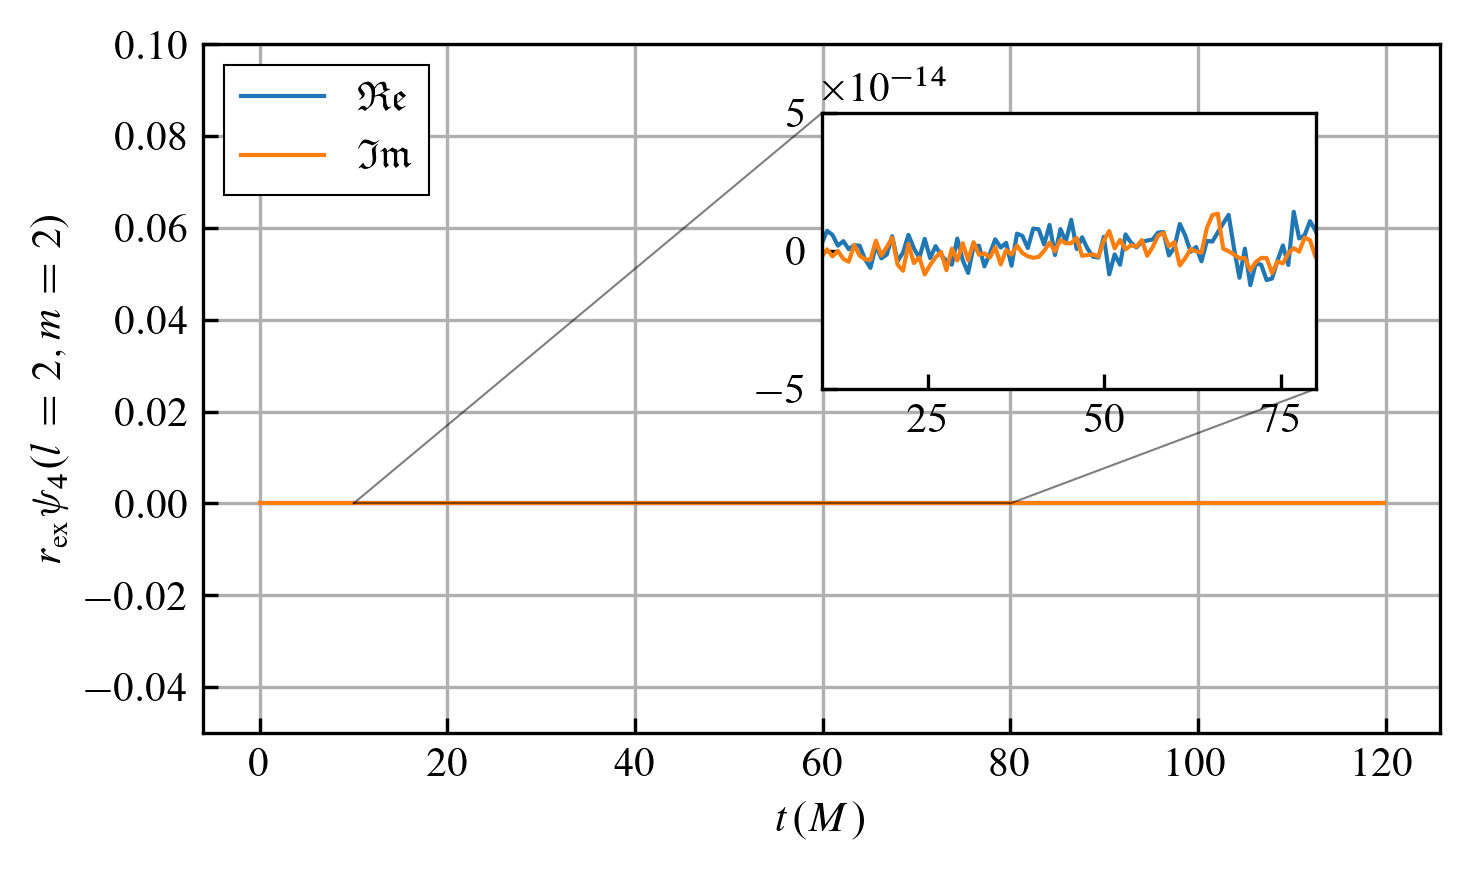
\includegraphics[width=0.5\textwidth]{data/psi4_r50.png}% Here is how to import EPS art
%	\caption{\label{fig:psi4_r50} Real part and imaginary part of $r_\mathrm{ex}\psi_4$. Red dashed line indicates $r=r_\mathrm{ex}=50M$.}
%\end{figure}

\section{Result}

\subsection{Gravitational Waves}

For wave extraction, we utilized the \textsc{WeylScal4} and \textsc{Multipole} thorns \cite{Baker:2001sf}. These thorns extract the Weyl scalar and decompose it into the spin-weighted spherical harmonics. To calculate the radiated energy, we considered modes up to $l=8$, which are considered credible because higher modes are dominated by numerical noise \cite{Pollney:2009yz}.

Since the Schwarzschild metric has spherical symmetry, there should be no gravitational wave radiation. Figure~\ref{fig:psi4_r50} displays the real and imaginary parts of $r_\mathrm{ex}\psi_4$. There is no notable difference between $r_\mathrm{ex} = 50M$. Furthermore, all values of $r_\mathrm{ex}\psi_4$ are on the order of $10^{-14}$, which can be regarded as numerical noise.

\begin{figure}[h]
	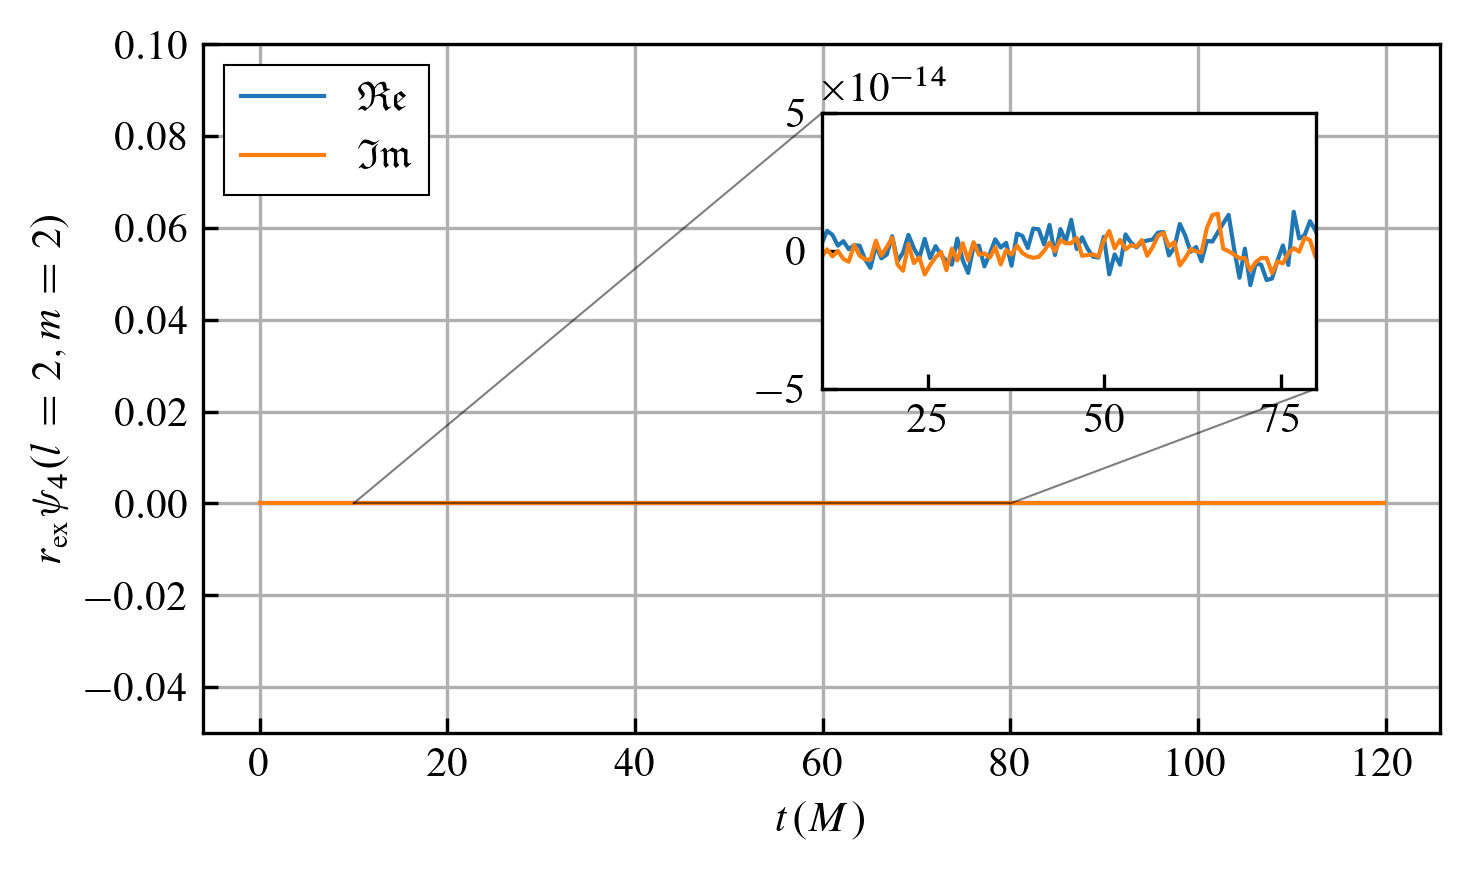
\includegraphics[width=0.5\textwidth]{data/psi4_r50.png}% Here is how to import EPS art
	\caption{\label{fig:psi4_r50} Real and imaginary parts of $r_\mathrm{ex}\psi_4$. The red dashed line indicates $r=r_\mathrm{ex}=50M$.}
\end{figure}



\subsection{Apparent Horizon}

We measured apparent horizon at each time using \textsc{AHFinderDirect} \cite{Thornburg:1995cp, Thornburg:2003sf}. It finds an apparent horizon by numerically solving equation
\begin{eqnarray}
	\Theta &\equiv & D_i n^i + K_{ij} n^i n^j - K = 0,
\end{eqnarray}
where $n^i$ is the outward-pointing unit normal to the apparent horizon, and $D_i$ is the covariant derivative operator associated with the 3-metric in the slice.

We don't fixed puncture location at the origin, but there was no puncture moving and the puncture still at the origin. Fig.~\ref{fig:expansion} shows expansion of apparent horizon as function of time. Fig.~\ref{fig:m_irr} shows irreducible mass as function of time. 

\begin{figure}[h]
	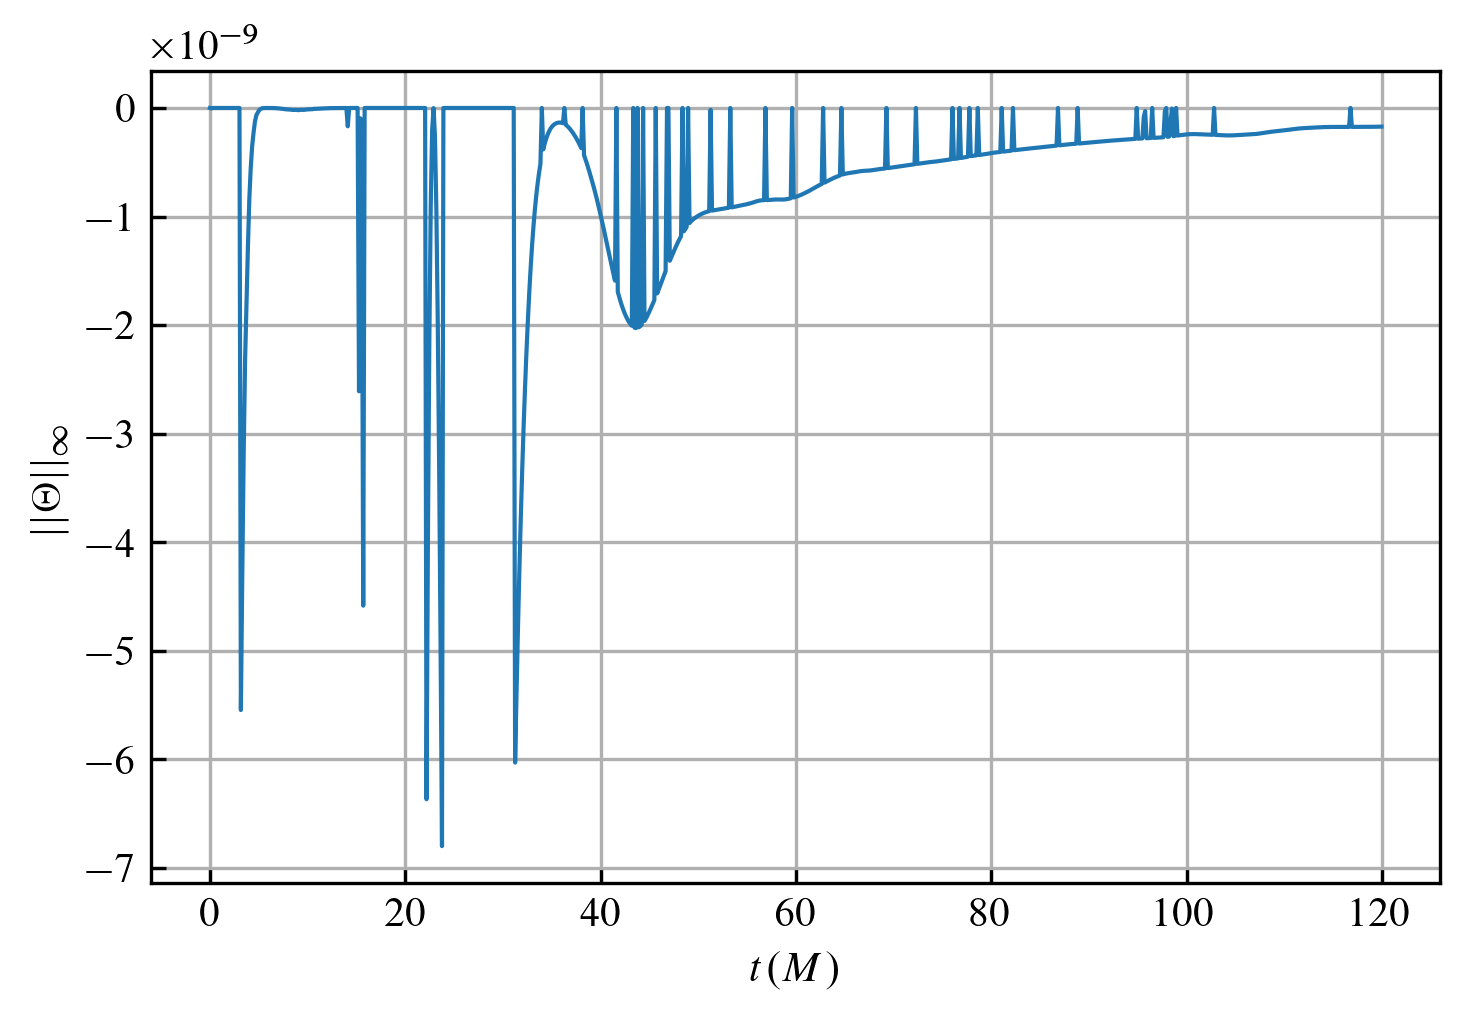
\includegraphics[width=0.5\textwidth]{data/expansion.png}% Here is how to import EPS art
	\caption{\label{fig:expansion} Expansion $\Theta$ of apparent horizon as function of time.}
\end{figure}

\begin{figure}[h]
	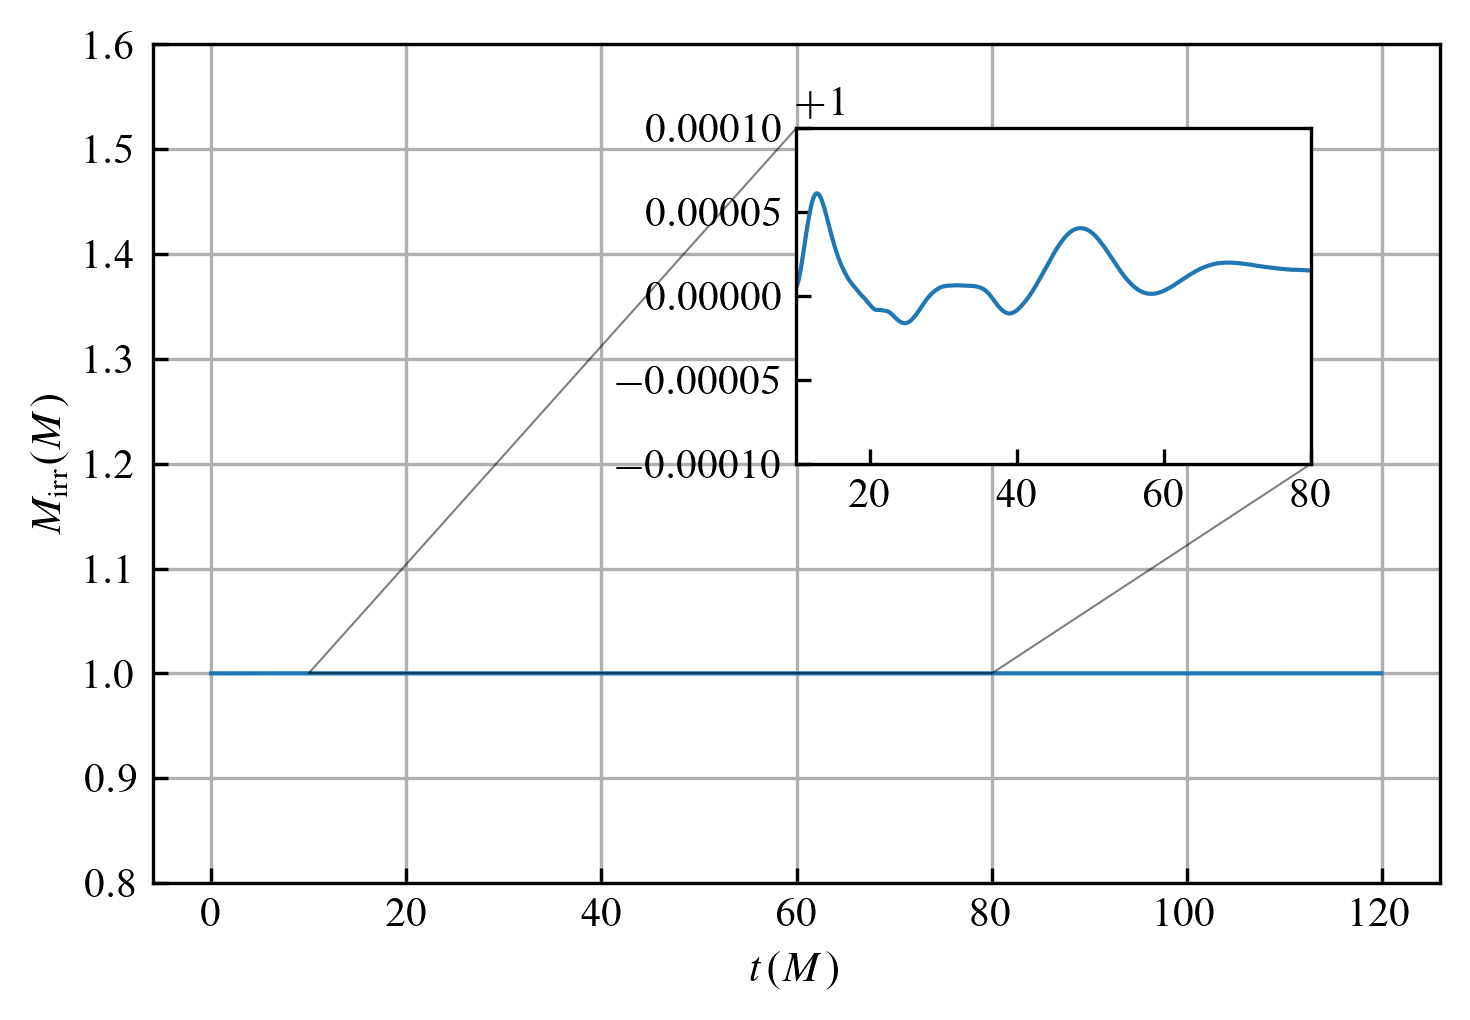
\includegraphics[width=0.5\textwidth]{data/m_irr.png}% Here is how to import EPS art
	\caption{\label{fig:m_irr} Irreducible mass $M_\mathrm{irr}$ as function of time.}
	\end{figure}

%\nocite{*}

\bibliography{eintk}% Produces the bibliography via BibTeX.


\end{document}
%
% ****** End of file apssamp.tex ******
